\documentclass[final]{siamltex}

% for red MarginPars
\usepackage{color}

% for \boldsymbol
\usepackage{amsmath}

\usepackage{latexsym}
\usepackage{graphicx}
\usepackage{geometry}
\usepackage{hyperref}

% total number of floats allowed on a page
\setcounter{totalnumber}{100}

% MarginPar
\setlength{\marginparwidth}{0.75in}
\newcommand{\MarginPar}[1]{\marginpar{\vskip-\baselineskip\raggedright\tiny\sffamily\hrule\smallskip{\color{red}#1}\par\smallskip\hrule}}

% for non-stacked fractions
\newcommand{\sfrac}[2]{\mathchoice
  {\kern0em\raise.5ex\hbox{\the\scriptfont0 #1}\kern-.15em/
   \kern-.15em\lower.25ex\hbox{\the\scriptfont0 #2}}
  {\kern0em\raise.5ex\hbox{\the\scriptfont0 #1}\kern-.15em/
   \kern-.15em\lower.25ex\hbox{\the\scriptfont0 #2}}
  {\kern0em\raise.5ex\hbox{\the\scriptscriptfont0 #1}\kern-.2em/
   \kern-.15em\lower.25ex\hbox{\the\scriptscriptfont0 #2}}
  {#1\!/#2}}

\newcommand{\V}[1]{\boldsymbol{#1}}

\def\Ab {{\bf A}}
\def\bb {{\bf b}}
\def\fb {{\bf f}}
\def\Ib {{\bf I}}
\def\Mb {{\bf M}}
\def\Pb {{\bf P}}
\def\rb {{\bf b}}
\def\ub {{\bf u}}
\def\xb {{\bf x}}

\def\deltab {\boldsymbol{\delta}}
\def\phib {\boldsymbol{\phi}}
\def\taub   {\boldsymbol{\tau}}

\begin{document}

%==========================================================================
% Title
%==========================================================================
\title{Notes for the Preconditioned GMRES Algorithm}

\maketitle

\section{General Form}
This code solve the following linear system using a preconditioned GMRES algorithm:
\begin{equation}
\underbrace{
\left(\begin{array}{cc}
\mathcal{A} & \mathcal{G} \\
-\mathcal{D} & 0
\end{array}\right)
}_{\Ab}
\underbrace{
\left(\begin{array}{c}
\xb_{\ub} \\
x_p
\end{array}\right)
}_{\xb}
=
\underbrace{
\left(\begin{array}{c}
\bb_{\ub}\\
b_p
\end{array}\right)}_{\bb},\label{eq:Ax=b}
\end{equation}
where $\xb_\ub$ and $\bb_\ub$ are staggered quantities and $x_p$ and $b_p$ are
cell-centered quantities.  The gradient operator, $\mathcal{G}$, operates on
cell-centered data and returns a staggered field.  The divergence operator, 
$\mathcal{D}$, operates on staggered data and returns a cell-centered field.  
The Helmholtz-like operator, $\mathcal{A}$, has the general form,
$\mathcal{A} = \Theta\alpha\mathcal{I} - \mathcal{A}_0$, where
$\Theta$ is a constant parameter,
$\alpha$ is a cell-centered quantity,
$\mathcal{I}$ is the identity matrix, 
and $\mathcal{A}_0$ represents the viscous stress tensor.
Both $\mathcal{A}$ and $\mathcal{A}_0$ operate on staggered data and return
a staggered field.\\

The code has several options for the viscous stress tensor.  For ease of exposition,
we define $\mathcal{A}_0$ as a function of a velocity vector, $\ub$:\\
\begin{itemize}
\item $|${\tt visc\_type}$|$=1 $\quad\rightarrow\quad \mathcal{A}_0(\ub) = \nabla\cdot\beta\nabla\ub$.\\
\item $|${\tt visc\_type}$|$=2 $\quad\rightarrow\quad \mathcal{A}_0(\ub) = \nabla\cdot\left\{\beta[\nabla\ub + (\nabla\ub)^T]\right\}$.\\
\item $|${\tt visc\_type}$|$=3 $\quad\rightarrow\quad \mathcal{A}_0(\ub) = \nabla\cdot\left\{\beta[\nabla\ub + (\nabla\ub)^T] + \mathcal{I}\left(\gamma - \frac{2}{3}\beta\right)(\nabla\cdot\ub)\right\}$.\\
\end{itemize}
If {\tt visc\_type} is positive, we assume that $\alpha, \beta$, and $\gamma$ are constant
in space, and use simplified stencils for efficiency.

\section{Preconditioner Algorithm}

We shall denote the preconditioner as $\Mb^{-1}$, which is an approximation
for $\Ab^{-1}$.  The evaluation of $\Mb^{-1}\bb$ can be divided
into three steps:\\

\begin{itemize}
\item {\it Step 1:} Compute an intermediate solution, $\xb_{\ub}^*$, using an implicit viscous solve.\\ \\
We solve the following equation for $\xb_{\ub}^*$:
\begin{equation}
\mathcal{A} \xb_{\ub}^* \equiv (\Theta\alpha\mathcal{I} - \mathcal{A}_0)\xb_{\ub}^* = \bb_{\ub}.\label{eq:viscous solve}
\end{equation}

\item {\it Step 2:} Form the right-hand-side of a pressure Poisson problem.\\ \\
We wish to solve the following equation for $\Phi$:
\begin{equation}
\mathcal{L}_\alpha\Phi = \mathcal{D}\xb_\ub^* + b_p\label{eq:Poisson}
\end{equation}
To derive this equation, we first state that
we wish to solve for some $\xb_\ub$ and $\phi$ such that
\begin{equation}
\mathcal{A}\xb_\ub + \mathcal{G}\phi = \bb_\ub,\label{eq:proj phi}
\end{equation}
subject to equation (\ref{eq:viscous solve}) and preservation of viscous balance,
i.e., $\mathcal{A}_0\xb_\ub^* = \mathcal{A}_0\xb_\ub$.
Subtracting (\ref{eq:viscous solve}) from (\ref{eq:proj phi}) and applying
the viscous balance condition, we obtain
\begin{equation}
\Theta\alpha\mathcal{I}(\xb_\ub-\xb_\ub^*) + \mathcal{G}\phi = 0,
\end{equation}
or equivalently,
\begin{equation}
\xb_\ub-\xb_\ub^* + (\alpha\mathcal{I})^{-1}\mathcal{G}\Phi = 0,\label{eq:proj phi 2}
\end{equation}
with $\Phi = \phi/\Theta$.  Taking the divergence of both sides, we obtain (\ref{eq:Poisson})\\

\item {\it Step 3:} Compute $\xb_\ub$ and $x_p$.\\

We begin by solving (\ref{eq:Poisson}) for $\Phi$.  Next, 
by rearranging (\ref{eq:proj phi 2}), we obtain
\begin{equation}
\xb_{\ub} = \xb_{\ub}^* - (\alpha\mathcal{I})^{-1}\mathcal{G}\Phi.\label{eq:x_b update}
\end{equation}
We compute $x_p$ using:
\begin{equation}
x_p = (\Theta\mathcal{I} - \chi\mathcal{L}_\alpha)\Phi,\label{eq:x_p}
\end{equation}
where
\begin{equation}
\chi =
\begin{cases}
\beta, & {\rm |visc\_type|} = 1\\
2\beta, & {\rm |visc\_type|} = 2\\
\frac{4}{3}\beta + \gamma, & {\rm |visc\_type|} = 3
\end{cases}
\end{equation}
In Section \ref{sec:projection} we provide a derivation of (\ref{eq:x_p}),
and describe under what conditions the pressure is computed exactly.\\

A more preferred variation that is analytically equivalent
to (\ref{eq:x_p}) if (\ref{eq:Poisson}) is solved exactly:
\begin{eqnarray}
x_p &=& \Theta\mathcal{I}\Phi - \chi(\mathcal{D}\xb_\ub^* + b_p).
\end{eqnarray}
This is slightly more computationally efficient than (\ref{eq:x_p}),
and in our testing makes the overall
GMRES algorithm converge faster when we (intentionally) perform a small
number of V-cycles for the Poisson solver.\\

\end{itemize}

These steps can be represented as the following operator:
\begin{equation}
\Mb^{-1}_1\bb =
\underbrace{
\left(\begin{array}{cc}
\mathcal{I} & -(\alpha\mathcal{I})^{-1}\mathcal{G} \widetilde{\mathcal{L}_{\alpha}}^{-1} \\
0  & \Theta \widetilde{\mathcal{L}_{\alpha}}^{-1} - \chi\mathcal{I}
\end{array}\right)
}_{\rm{\it Step~3}}
\underbrace{
\left(\begin{array}{cc}
\mathcal{I} & 0\\
\mathcal{D} & \mathcal{I}
\end{array}\right)
}_{\rm{\it Step~2}}
\underbrace{
\left(\begin{array}{cc}
\mathcal{A}^{-1} & 0\\
0 & \mathcal{I}
\end{array}\right)
}_{\rm{\it Step~1}}
\bb.
\end{equation}
Here, we denote with $\widetilde{\mathcal{L}_{\alpha}}^{-1} $, the inverse of $\mathcal{L}_{\alpha}$ approximately 
calculated via multigrid. By this way of updating pressure, one can avoid the calculation for ${\mathcal{L}_{\alpha}}$. 
The less efficient preconditioner takes the form
\begin{equation}
\widetilde{\Mb}_1^{-1}\bb =
\underbrace{
\left(\begin{array}{cc}
\mathcal{I} & -(\alpha\mathcal{I})^{-1}\mathcal{G} \widetilde{\mathcal{L}_\alpha}^{-1}\\
0 & (\Theta\mathcal{I} - \chi\mathcal{L}_\alpha) \widetilde{\mathcal{L}_\alpha}^{-1}
\end{array}\right)
}_{\rm{\it Step~3}}
\underbrace{
\left(\begin{array}{cc}
\mathcal{I} & 0\\
\mathcal{D} & \mathcal{I}
\end{array}\right)
}_{\rm{\it Step~2}}
\underbrace{
\left(\begin{array}{cc}
\mathcal{A}^{-1} & 0\\
0 & \mathcal{I}
\end{array}\right)
}_{\rm{\it Step~1}}
\bb.
\end{equation}
When the inverse of $\mathcal{L}_\alpha$ is inexactly approximated, we see that two ways of updating pressure are different. 

\subsection{Notes on the Projection Formulation}\label{sec:projection}
Here we derive equation (\ref{eq:x_p}).  First, apply $\mathcal{A}$ to (\ref{eq:x_b update}):
\begin{equation}
\mathcal{A}\xb_{\ub} - \mathcal{A}\xb_{\ub}^* = -\mathcal{A}(\alpha\mathcal{I})^{-1}\mathcal{G}\Phi.
\end{equation}
From (\ref{eq:Ax=b}) we know $\mathcal{A}\xb_{\ub} = \bb_{\ub} - \mathcal{G} x_p$, 
and also noting (\ref{eq:viscous solve}), we have:
\begin{eqnarray}
\mathcal{G} x_p &=& \mathcal{A}(\alpha\mathcal{I})^{-1}\mathcal{G}\Phi\nonumber\\
&=& \left(\Theta\alpha\mathcal{I} - \mathcal{A}_0\right)(\alpha\mathcal{I})^{-1}\mathcal{G}\Phi\nonumber\\
&=&\Theta\mathcal{G}\Phi -\mathcal{A}_0(\alpha\mathcal{I})^{-1}\mathcal{G}\Phi.
\end{eqnarray}
Applying $\mathcal{L}^{-1}\mathcal{D}$ to both sides, we have:
\begin{eqnarray}
x_p &=& \Theta\mathcal{L}^{-1}\mathcal{D}\mathcal{G}\Phi - \mathcal{L}^{-1}\mathcal{D}\mathcal{A}_0(\alpha\mathcal{I})^{-1}\mathcal{G}\Phi\nonumber\\
&=& \Theta\Phi - \mathcal{L}^{-1}\mathcal{D}\mathcal{A}_0(\alpha\mathcal{I})^{-1}\mathcal{G}\Phi.
\end{eqnarray}
We are now going to make the following assumptions:\\
\begin{itemize}
\item We will assume that $\mathcal{A}_0 = \beta\mathcal{L}$.  Note that this also 
assumes $\beta$ is constant, and therefore $\beta$ and $\mathcal{L}$ commute.
Note that for {\tt visc\_type} $=1$, these assumptions are true.
These assumptions are also true if {\tt visc\_type} $>1$ and $b_p=0$.\\
\item We will assume that $\mathcal{D}$ and $\mathcal{L}$ commute.  Note that this 
assumption is true for periodic problems.\\
\end{itemize}
Altogether, we arrive at:
\begin{equation}
x_p = \Theta\Phi - \beta\mathcal{L}_\alpha\Phi = \left(\Theta\mathcal{I} - \beta\mathcal{L}_\alpha\right)\Phi.
\end{equation}

We can show that the preconditioner solves the problem exactly, i.e. $\Mb^{-1}\Ab = \Ib$,
under certain conditions.  Without any assumptions, if $\widetilde{\mathcal{L}_\alpha}^{-1}=\mathcal{L}_\alpha^{-1}$,
\begin{equation}
\Mb_1^{-1}\Ab =
\left(\begin{array}{cc}
\mathcal{I} & \mathcal{G}\mathcal{A}^{-1}[\mathcal{I}-\mathcal{D}\mathcal{L}_\alpha^{-1}(\alpha\mathcal{I})^{-1}\mathcal{G}]\\
0 & \mathcal{D}\mathcal{G}\mathcal{A}^{-1}\mathcal{L}_\alpha^{-1}(\Theta\mathcal{I}-\chi\mathcal{L}_\alpha)
\end{array}\right).
\end{equation}
If we assume $\alpha$ is constant and the problem is periodic (so $\mathcal{D}$ 
and $\mathcal{L}_\alpha^{-1}$ commute), then the upper-right entry becomes zero.  If 
we also assume $\beta$ is constant, then $\mathcal{A}^{-1}$ and $\mathcal{L}_\alpha^{-1}$ 
commute and it can be shown that lower-right entry becomes the identity if 
$\mathcal{A}_0=\beta\mathcal{L}$, i.e., {\tt visc\_type}=+1.

\subsection{Notes on the Preconditioners Selection}\label{sec:preconditioners}

\begin{itemize}
\item $|${\tt precon\_type}$|$=1 $\quad\rightarrow\quad \mbox{Projection preconditioners}: {\Mb_1}~\mbox{or}~\widetilde{\Mb}_1$.\\
\item $|${\tt precon\_type}$|$=2 $\quad\rightarrow\quad \mbox{Lower triangular preconditioners}: {\Mb_2}$.\\
\item $|${\tt precon\_type}$|$=3 $\quad\rightarrow\quad \mbox{Upper triangular preconditioners}: {\Mb_3}$.\\
\item $|${\tt precon\_type}$|$=4 $\quad\rightarrow\quad \mbox{Block diagonal preconditioners}: {\Mb_4}$.\\
\end{itemize}
In projection preconditioners, if ${\tt precon\_type}=-1$, it means using $\widetilde{\Mb}_1^{-1}$ for updating pressure term;
if  ${\tt precon\_type}=1$, it means using ${\Mb_1}^{-1}$ in pressure update. For ${\Mb_2}, {\Mb_3}, {\Mb_4}$, if negative sign 
is chosen (${\tt precon\_type}=-2, -3, -4$), it means that putting a negative sign in front of the pressure Schur complement approximations.
Define $s = \mbox{sign} ({\tt precon\_type})$.\\ \\

For $\Mb^{-1}_2\bb$ the steps are as follows:
\begin{itemize}
\item {\it Step 1:} Compute $\xb_{\ub}$, using an implicit viscous solve.
\item {\it Step 2:} Form the right-hand-side of a pressure Poisson problem.
\item {\it Step 3:} Compute $x_p$.
\end{itemize}
\begin{equation}
\Mb^{-1}_2\bb =
\underbrace{
\left(\begin{array}{cc}
\mathcal{I} & 0 \\
0 & s(\Theta \widetilde{\mathcal{L}_\alpha}^{-1} - \chi \mathcal{I}) 
\end{array}\right)
}_{\rm{\it Step~3}}
\underbrace{
\left(\begin{array}{cc}
\mathcal{I} & 0\\
\mathcal{D} & \mathcal{I}
\end{array}\right)
}_{\rm{\it Step~2}}
\underbrace{
\left(\begin{array}{cc}
\mathcal{A}^{-1} & 0\\
0 & \mathcal{I}
\end{array}\right)
}_{\rm{\it Step~1}}
\bb.
\end{equation}

For $\Mb^{-1}_3\bb$ the steps are as follows:
\begin{itemize}
\item {\it Step 1:} Compute $x_p$.
\item {\it Step 2:} Compute $\xb_{\ub}^*$.
\item {\it Step 3:} Compute $\xb_{\ub}$ using an implicit viscous solve.
\end{itemize}
\begin{equation}
\Mb^{-1}_3\bb =
\underbrace{
\left(\begin{array}{cc}
\mathcal{A}^{-1} & 0\\
0 & \mathcal{I}
\end{array}\right)
}_{\rm{\it Step~3}}
\underbrace{
\left(\begin{array}{cc}
\mathcal{I} & -\mathcal{G}\\
0 & \mathcal{I}
\end{array}\right)
}_{\rm{\it Step~2}}
\underbrace{
\left(\begin{array}{cc}
\mathcal{I} & 0 \\
0 & s(\Theta \widetilde{\mathcal{L}_\alpha}^{-1}- \chi \mathcal{I}) 
\end{array}\right)
}_{\rm{\it Step~1}}
\bb.
\end{equation}

\begin{equation}
\Mb^{-1}_4\bb =
\left(\begin{array}{cc}
\mathcal{A}^{-1} & 0\\
0 & -s\chi \mathcal{I} 
\end{array}\right)
\bb.
\end{equation}

$\Mb^{-1}_5\bb$: First do $\Mb^{-1}_2\bb$ to obtain $x_p$ and a preliminary solution,
for $\xb_{\ub}^*$.  Then, solve for $\xb_{\ub} = \mathcal{A}^{-1}(\bb_{\ub} - \mathcal{G}x_p)$
using $\xb_{\ub}^*$ as an initial guess.

\section{Boundary Conditions}

We have two types of non-periodic boundary conditions, {\tt SLIP} and {\tt NO\_SLIP}.
Both of these boundary conditions imply a Dirichlet condition on normal velocity.
The {\tt SLIP} condition implies a Dirichlet traction condition that
is used to derive a Neumann condition on the transverse velocity.
The {\tt NO\_SLIP} condition implies a Dirichlet velocity condition for the
transverse velocity.  By default all boundary conditions are assumed to be homogeneous.
We we use the {\tt prob\_sol} flag to apply inhomogeneous boundary conditions for
filling ghost cells.

We summarize our philosophy of ghost cells for the {\tt SLIP} and {\tt NO\_SLIP}
conditions.  Here, we use ``velocity'' to refer to $\xb_{\ub}$ and ``pressure'' to refer
to $x_p$.

\begin{itemize}

\item For normal velocity, the value on the boundary is obviously some prescribed Dirichlet
value.  We take the approach that values behind these ghost edges shall not affect
the solution.\\

\item For transverse velocity, we use the convention that the values in ghost edges correspond
to extrapolations to the ghost edge.  These ghost cells are filled using two point
stencils that include the interior value and the boundary condition.
Traction condition means that the shear stress (off-diagonal component in $\taub$)
is set to some prescribed value.  In 2D, for {\tt visc\_type=2},
\begin{equation}
\eta\left(\frac{\partial u}{\partial y} + \frac{\partial v}{\partial x}\right) = \text{prescribed Dirichlet}.
\end{equation}
Thus, this stencil will also include values of the normal velocity on the wall.

\item For pressure and $\Phi$, we use the convention that the values in ghost edges 
correspond to extrapolations to the ghost cell.  For {\tt SLIP} and {\tt NO\_SLIP} the only
possible physical condition is $\partial\phi/\partial n = 0$, so we simply copy
the interior value (which corresponds to a two point stencil involving the interior
point and the boundary condition).\\

\item For $\alpha, \beta$, and $\gamma$, we use the convention that the values in ghost cells
correspond to the values on the boundary.  When $\alpha, \beta$, and $\gamma$ are a
function of space, during initialization we fill these values as if they represent
the value in the ghost cell-centered, then call a routine to overwrite the ghost cells
to be the value averaged to the boundary.

\end{itemize}

\subsection{Inhomogeneous Boundary Conditions}
In practice, whenver we wish to solve (\ref{eq:Ax=b}) with inhomogeneous boundary
conditions, we use a residual correction technique to convert the problem to one
with homogeneous boundary conditions of the same type (Neumann or Dirichlet, based on the
choice of {\tt SLIP} or {\tt NO\_SLIP}):
\begin{equation}
\Ab_H\xb = \bb - \Ab\xb_H.
\end{equation}
Here, $\Ab_H$ is the same operator as $\Ab$, but with homogeneous boundary conditions.
The vector $\xb_H$ is a vector with zeros in all valid cells (but possibly
non-zero values in the ghost cells, depending on the boundary conditions).
By solving this system for $\xb$, we arrive at the same answer as solving the
inhomogeneous problem, $\Ab\xb=\bb$.

\section{Code Control}

\subsection{Code control, init\_mat} The coefficient matrix is controled by 
prob\_coeff:
 
1. density=1, viscosity=1, $\gamma=1$.

2. density=1, viscosity=random, $\gamma=1$.

3. density=random, viscosity=1, $\gamma=1$.

4. random density and random viscosity

5. density=1, smooth viscosity
$$
\mu(x,y)=1+\frac{1}{2} \mbox{cos}(2 \pi x) \mbox{sin}(2 \pi y).
$$

6. Density and viscosity distribute like a bubble, smoothed by $\mbox{tanh}$ near the interface. Default density ratio: $2:4$, default 
viscosity ratio: $2:4$ (can be adjusted, if one wants to increase the density/viscosity ratios).   

7. Density and viscosity distribution has bilayers, smootheed by by $\mbox{tanh}$ near the interface. density ratio: $1:3$, viscosity ratio: $1:3$.  (can be adjusted, if one wants to increase the density/viscosity ratios). 

\subsection{Code control: prob\_sol} To control the initial solution, the right hand side. Some cases: 

{\bf Case (1).} Let the domain be $[0, L_x] \times [0, L_y]$, where $L_x=L_y==L=2^{6}$. We fix $\mu =1$, $h_x=h_y=h=1$ and $\Delta t= 0.5 \frac{h^2}{\mu }= 0.5$. 
Boundary conditions are provided by the solution of the Taylor vortex flow with constant
$\mu$ and $\rho=1$:
\begin{equation}\label{TaylorVortex}
 \left \{
  \begin{array} {lll}
u({\bf x}, t)&=1 - 2e^{-8\pi^2\mu t/L^2}\cos{\left(\frac{2\pi(x-t)}{L}\right)}\sin{\left(\frac{2\pi(y-t)}{L}\right)},  \\
v({\bf x}, t)&=1 + 2e^{-8\pi^2\mu t/L^2}\sin{\left(\frac{2\pi(x-t)}{L}\right)}\cos{\left(\frac{2\pi(y-t)}{L}\right)}, \\
p({\bf x}, t)&= -e^{-16\pi^2\mu t/L^2}\left[\cos{\left(\frac{4\pi(x-t)}{L}\right)} + \cos{\left(\frac{4\pi(y-t)}{L}\right)}\right].
  \end{array}
 \right.
\end{equation}
(\ref{TaylorVortex}) is the solution of unforced Navier-Stokes equation.
Divergence free. 

{\bf Case (2).} ABC flow in 3D case. 

{\bf Case (3).} We test a density=1, {\bf variable viscosity example with analytic solution}: % (Maple file: new\_model6.mw):
$$
u=\mbox{e}^{(-8\pi^2t)}\mbox{sin}(2 \pi x)\mbox{sin}(2 \pi y); \quad v=\mbox{e}^{(-8\pi^2t)}\mbox{cos}(2 \pi x)\mbox{cos}(2 \pi y);
$$
$$
p=\mbox{e}^{(-16 \pi^2 t)}(\mbox{cos}(4 \pi x)+\mbox{cos}(4 \pi y));
\quad
\mu(x,y)=1+\frac{1}{2} \mbox{cos}(2 \pi x) \mbox{sin}(2 \pi y).
$$
Here, $\mu(x,y)$ is used to evaluate the viscosity at cell centers (we also use analytic function to evaluate the viscosity at cell nodes).
If strain form viscous term is used, then 
$$
\begin{array} {ll}
f_1=4 \pi \mbox{e}^{-8 \pi^2 t} (-2 \mbox{sin}(2 \pi x) \pi \mbox{cos}(2 \pi x)+2 \mbox{sin}(2 \pi x) \pi \mbox{cos}(2 \pi x) \mbox{cos}(2 \pi y)^2+\mbox{e}^{-8 \pi^2 t} \mbox{sin}(4 \pi x))
\\
f_2=4 \pi \mbox{e}^{-8 \pi^2 t} (2 \mbox{cos}(2 \pi x)^2 \mbox{cos}(2 \pi y) \pi \mbox{sin}(2 \pi y)-\mbox{e}^{-8 \pi^2 t} \mbox{sin}(4 \pi y))
\end{array}
$$
Divergence free flow.
%The computational domain is % $[0, 1]^2$. We let $\Delta t$ ($\Delta t  \propto {h_x^2}$) vary so that the viscous CFL number varies.

{\bf Case (6).} Incompressible mode. Constant coefficient mode with boundary conditions imposed as $x$- direction periodic, $y$-direction Dirichlet.


{\bf Case (100).} random initial solution, both density and viscosity are constant and equal to 1. Steady state problem with Laplacian viscous term.
the RHS is generated by using apply\_matrix, initial solutions are set to be the mean values of the exact solution (random) 


{\bf Case (31).} For testing discretization accuracy of stencils. The density=1, smooth viscosity generated by case(5) in init\_mat. 
The velocity solution is smooth but not divergence free and rhs is controled by prob\_sol=31. 

\section{Multigrid}
We employ a standard V-cycle multigrid approach (cite Briggs ``Multigrid Tutorial'') for
both the ``cell-centered'' multigrid solver for the weighted Poisson problem and the
``staggered'' multigrid solver for the viscous operator.  We refer to the solver in this
way because the cell-centered solver computes a cell-centered $\Phi$, whereas the
staggered solver computed staggered velocity componentns.
Since our multigrid solves are one component of a preconditioned
GMRES algorithm, we do not solve the problem to a tolerance-based completion, 
but rather perform a fixed number of V-cycles per solve.

Multigrid consists of 3 major components: (i) choice of relaxation at a particular level,
(ii) coarsening/restriction operator, and (iii) interpolation/prolongation operator.
For the bottom (coarsest-level) solve, we perform a specified number of relaxations
rather than use a more elaborate iterative solver, so that we guarantee that each
application of the preconditioner retains the same symbol.  We use the standard residual
formulation, so that on all coarsened levels we are solving for the error in the
coarsened residual from the next-finer level.

%%%%%%%%%%%%%%%%%%%%%%%%%%%%%%%%%
\begin{figure}[tb]
\centering
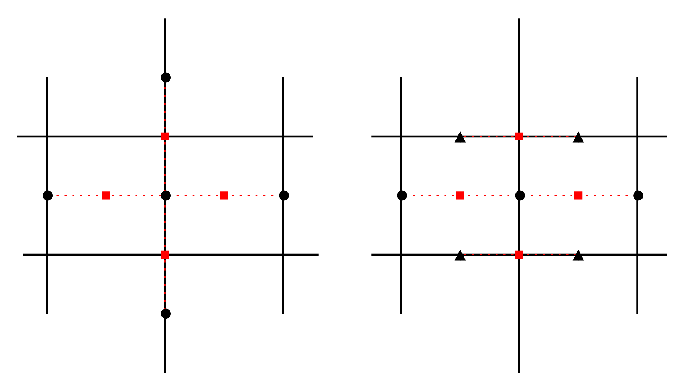
\includegraphics[width=3.5in]{viscOp}
\label{fig:viscOp}
\caption{The stencils for the $x$-component of (Left) $\nabla\cdot\beta\nabla\phib$ and 
(Right) $\nabla\cdot\beta(\nabla\phib)^T$.  
The black circles indicate locations of $u$.
The black triangles indicate locations of $v$.
The red dots indicate the location of the $\beta$ and the gradients of velocity.}
\end{figure}
%%%%%%%%%%%%%%%%%%%%%%%%%%%%%%%%%
%%%%%%%%%%%%%%%%%%%%%%%%%%%%%%%%%
\begin{figure}[tb]
\centering
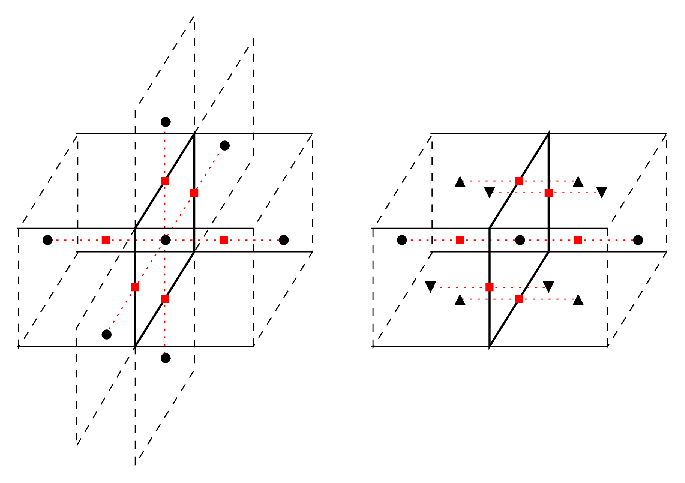
\includegraphics[width=3.5in]{viscOp_3d}
\label{fig:viscOp_3d}
\caption{The stencils for the $x$-component of (Left) $\nabla\cdot\beta\nabla\phib$ and
(Right) $\nabla\cdot\beta(\nabla\phib)^T$.  
The black circles indicate locations of $u$.
The black triangles indicate locations of $v$ and $w$.
The red dots indicate the location of the $\beta$ and the gradients of velocity.}
\end{figure}
%%%%%%%%%%%%%%%%%%%%%%%%%%%%%%%%%

{\bf Relaxation.}  Both the staggered and cell-centered solvers use a Gauss-Seidel
varient with unity weighting factor, $\omega$.  Th cell-centered solver uses standard red-black
relaxation, whereas the staggered solver uses a 2$D$-colored relaxation,
where $D$ is the dimensionality of the problem.  In particular, we order the relaxations
as follows: red-x, black-x, red-y, black-y, red-z, black-z.
Given a cell-centered operator of the form,
$\nabla\cdot\beta\nabla\phi \equiv \mathcal{L}\phi = r$,
or a staggered operator of the form,
$\alpha\phi - \nabla\cdot\beta[\nabla\phi + (\nabla\phi)^T] \equiv \mathcal{L} \phi = r$,
the relaxation takes the form,
\begin{equation}
\phi^{k+1} = \phi^k + \omega\mathcal{D}^{-1}(r-\mathcal{L}\phi^k),
\end{equation}
where the superscript represents the iterate, and $\mathcal{D}^{-1}$ is the inverse of the
diagonal elements of $\mathcal{L}$.

{\bf Restriction.}  For the cell-centered solver, restriction is a simple averaging of
the $2^D$ fine cells.  For the staggered solver, we use a slightly more complicated
6-point (2D) or 12-point (3D) stencil.  For example, for x-faces we use
\begin{equation}
\phi_{i,j}^{\rm c} = \frac{1}{8}\left(\phi_{2i-1,2j}^{\rm f}+\phi_{2i-1,2j+1}^{\rm f}+\phi_{2i+1,2j}^{\rm f}+\phi_{2i+1,2j+1}^{\rm f}\right) 
+ \frac{1}{4}\left(\phi_{2i,2j}^{\rm f}+\phi_{2i,2j+1}^{\rm f}\right)
\end{equation}

{\bf Prolongation.}  For the cell-centered solver, prolongation is simply direct
injection from the coarse cell to the overlaying $2^D$ fine cells.  For the
staggered solver, we use a slightly more complicated stencil that involves linear
interpolation for fine faces that overlay coarse faces, and bilinear interpolation
for fine faces that do not overlay coarse faces.  For example, for x-faces we use
\begin{equation}
\phi_{i,j}^{\rm f} = \frac{3}{4}\phi_{i/2,j/2}^{\rm c} + \frac{1}{4}\phi_{i/2,j/2-1}^{\rm c}, \quad \forall~i,j~{\rm both~even},
\end{equation}
\begin{equation}
\phi_{i,j}^{\rm f} = \frac{3}{8}\left(\phi_{i/2,j/2}^{\rm c}+\phi_{i/2+1,j/2}^{\rm c}\right) + \frac{1}{8}\left(\phi_{i/2,j/2-1}^{\rm c}+\phi_{i/2+1,j/2-1}^{\rm c}\right), \quad \forall~i~{\rm odd},j~{\rm even},
\end{equation}
where we use integer division in the index subscripts.





\end{document}
